% ============================================================
% Question Bank: ch06-03 Drawing Geometric Figures (Modified — IN)
% Topic Title: Drawing Geometric Figures with Given Conditions (IAS 2023 construction emphasis)
% CCSS: 7.G.A.2 (Modified for Indiana)
% Questions: 30 (18 MC + 7 SA + 5 Graphical)
% ============================================================

% --- Multiple Choice Questions (18) ---

\begin{practiceQuestion}{m-6-3-q01}{mc}
\begin{questionText}
A student constructs a triangle with sides $5$ cm, $7$ cm, and $3$ cm. Which step should come first?
\end{questionText}
\choiceA{Set the compass to $3$ cm and draw an arc}
\choiceB{Draw the longest side ($7$ cm) as the base}
\choiceC{Measure one of the angles with a protractor}
\choiceD{Connect the endpoints to form the triangle}
\correctAnswer{B}
\explanation{The first step in a standard construction is to draw one side as the base. Drawing the longest side ($7$ cm) first gives a stable foundation for the other arcs.}
\end{practiceQuestion}

\begin{practiceQuestion}{m-6-3-q02}{mc}
\begin{questionText}
When constructing a triangle with a compass and straightedge, why do you draw arcs from both endpoints of the base?
\end{questionText}
\choiceA{To measure the angles of the triangle}
\choiceB{To find the point that is the correct distance from both endpoints}
\choiceC{To make the drawing look more professional}
\choiceD{To check if the base is straight}
\correctAnswer{B}
\explanation{Each arc shows all points at a specific distance from an endpoint. The intersection of two arcs is the unique point at the correct distance from both endpoints.}
\end{practiceQuestion}

\begin{practiceQuestion}{m-6-3-q03}{mc}
\begin{questionText}
Can you draw a triangle with sides $4$ cm, $6$ cm, and $11$ cm?
\end{questionText}
\choiceA{Yes, and it is a unique triangle}
\choiceB{Yes, and there are many possible triangles}
\choiceC{No, because $4 + 6 = 10 < 11$}
\choiceD{No, because the sides are all different lengths}
\correctAnswer{C}
\explanation{The triangle inequality requires $4 + 6 > 11$. But $10 < 11$, so the arcs would never intersect. No triangle can be formed.}
\end{practiceQuestion}

\begin{practiceQuestion}{m-6-3-q04}{mc}
\begin{questionText}
A student draws a $6$ cm segment and then draws an arc of radius $4$ cm from one end and an arc of radius $5$ cm from the other. The arcs intersect twice. What does this mean?
\end{questionText}
\choiceA{Two different triangles can be formed}
\choiceB{The construction failed — no triangle is possible}
\choiceC{Both intersections produce congruent triangles (one is a mirror image)}
\choiceD{One intersection point is correct and the other is wrong}
\correctAnswer{C}
\explanation{The two intersection points produce mirror-image (reflected) versions of the same triangle. They are congruent — SSS still gives a unique triangle shape.}
\end{practiceQuestion}

\begin{practiceQuestion}{m-6-3-q05}{mc}
\begin{questionText}
Which justification explains why three valid side lengths (SSS) produce a unique triangle?
\end{questionText}
\choiceA{The triangle inequality guarantees it}
\choiceB{The arcs from both endpoints intersect at exactly one point (up to reflection)}
\choiceC{Three sides always make a right triangle}
\choiceD{The angles are already determined by the sides}
\correctAnswer{B}
\explanation{With three fixed lengths satisfying the inequality, the arcs intersect at exactly one point above the base (and one below, which is a mirror image). This determines one unique triangle.}
\end{practiceQuestion}

\begin{practiceQuestion}{m-6-3-q06}{mc}
\begin{questionText}
A rectangle has a perimeter of $20$ cm. How many different rectangles can be constructed?
\end{questionText}
\choiceA{None}
\choiceB{Exactly one}
\choiceC{Exactly two}
\choiceD{More than one}
\correctAnswer{D}
\explanation{The sides must add to $10$. Many dimension pairs work ($1 \times 9$, $2 \times 8$, $3 \times 7$, etc.), so multiple rectangles are possible.}
\end{practiceQuestion}

\begin{practiceQuestion}{m-6-3-q07}{mc}
\begin{questionText}
You are given two sides ($6$ cm and $8$ cm) and the included angle ($90°$). A student uses a protractor and ruler to construct the triangle. Which justification explains why the triangle is unique?
\end{questionText}
\choiceA{SSS — three sides are known}
\choiceB{ASA — two angles and the included side are known}
\choiceC{SAS — two sides and the included angle fix the triangle}
\choiceD{AAA — all angles are determined}
\correctAnswer{C}
\explanation{Two sides and the angle between them (SAS) fully determine one unique triangle. The protractor fixes the angle, and the ruler fixes the side lengths.}
\end{practiceQuestion}

\begin{practiceQuestion}{m-6-3-q08}{mc}
\begin{questionText}
A student uses dynamic geometry software to construct a triangle with sides $5$, $5$, and $5$. She drags a vertex. What happens?
\end{questionText}
\choiceA{The triangle changes shape freely}
\choiceB{The triangle stays equilateral but changes size}
\choiceC{The triangle cannot be dragged because it is fully determined}
\choiceD{The triangle becomes a different type (e.g., isosceles)}
\correctAnswer{C}
\explanation{With three fixed side lengths (SSS), the triangle is rigid. The software will not allow the vertex to be dragged to a different position while maintaining the constraints.}
\end{practiceQuestion}

\begin{practiceQuestion}{m-6-3-q09}{mc}
\begin{questionText}
Can a triangle have sides $2$, $5$, and $2$?
\end{questionText}
\choiceA{Yes, it is isosceles}
\choiceB{Yes, it is scalene}
\choiceC{No, because $2 + 2 < 5$}
\choiceD{No, because two sides are the same}
\correctAnswer{C}
\explanation{$2 + 2 = 4 < 5$. The triangle inequality fails. If you tried to construct it, the arcs would not intersect.}
\end{practiceQuestion}

\begin{practiceQuestion}{m-6-3-q10}{mc}
\begin{questionText}
Steps for constructing an equilateral triangle with side $6$ cm:
\begin{enumerate}
    \item Draw a $6$ cm segment $AB$.
    \item Set compass to $6$ cm. Draw an arc centered at $A$.
    \item Draw an arc centered at $B$ with the same radius.
    \item Mark the intersection point $C$. Connect $AC$ and $BC$.
\end{enumerate}
Which step ensures that $AC = 6$ cm?
\end{questionText}
\choiceA{Step 1}
\choiceB{Step 2}
\choiceC{Step 3}
\choiceD{Step 4}
\correctAnswer{B}
\explanation{In Step 2, the compass is set to $6$ cm centered at $A$. Every point on that arc is exactly $6$ cm from $A$. So the intersection point $C$ is $6$ cm from $A$.}
\end{practiceQuestion}

\begin{practiceQuestion}{m-6-3-q11}{mc}
\begin{questionText}
Which set of conditions for a quadrilateral allows more than one possible shape?
\end{questionText}
\choiceA{Four sides and four angles all specified}
\choiceB{Four side lengths only}
\choiceC{A quadrilateral with all right angles and side $5$ cm}
\choiceD{A square with diagonal $10$ cm}
\correctAnswer{B}
\explanation{Four side lengths alone do not fix the angles of a quadrilateral. Many shapes with different angles are possible.}
\end{practiceQuestion}

\begin{practiceQuestion}{m-6-3-q12}{mc}
\begin{questionText}
When using technology (e.g., GeoGebra) to construct a triangle, what advantage does it have over compass and straightedge?
\end{questionText}
\choiceA{It can construct shapes that are impossible with compass and straightedge}
\choiceB{It allows you to drag vertices to test if the shape is rigid (unique)}
\choiceC{It does not require the triangle inequality to hold}
\choiceD{It produces different triangles than physical construction}
\correctAnswer{B}
\explanation{Dynamic software lets you test uniqueness by dragging vertices. If the triangle is fully determined (e.g., SSS), dragging won't change it. If not (e.g., AAA), you can see it change size.}
\end{practiceQuestion}

\begin{practiceQuestion}{m-6-3-q13}{mc}
\begin{questionText}
Which of the following is NOT a valid justification for a construction step?
\end{questionText}
\choiceA{``All points on this arc are $5$ cm from vertex $A$''}
\choiceB{``I drew a straight line because it looks right''}
\choiceC{``The compass width ensures the side is exactly $8$ cm''}
\choiceD{``The protractor guarantees the angle is exactly $60°$''}
\correctAnswer{B}
\explanation{''It looks right'' is not a mathematical justification. Valid justifications reference specific measurements, tools, or geometric properties.}
\end{practiceQuestion}

\begin{practiceQuestion}{m-6-3-q14}{mc}
\begin{questionText}
A student claims that knowing three angles of a triangle ($50°$, $60°$, $70°$) is enough to construct exactly one triangle. Is the student correct?
\end{questionText}
\choiceA{Yes, three angles always determine a unique triangle}
\choiceB{No, because $50 + 60 + 70 \neq 180$}
\choiceC{No, three angles determine the shape but not the size}
\choiceD{Yes, but only if all angles are less than $90°$}
\correctAnswer{C}
\explanation{$50 + 60 + 70 = 180°$ \checkmark, but AAA only fixes the shape. Many triangles of different sizes share these angles. A side length is needed to fix the size.}
\end{practiceQuestion}

\begin{practiceQuestion}{m-6-3-q15}{mc}
\begin{questionText}
Which set of side lengths can form a triangle?
\end{questionText}
\choiceA{$1$, $2$, $4$}
\choiceB{$3$, $5$, $9$}
\choiceC{$4$, $6$, $9$}
\choiceD{$2$, $3$, $6$}
\correctAnswer{C}
\explanation{Check: $4 + 6 = 10 > 9$ \checkmark, $4 + 9 = 13 > 6$ \checkmark, $6 + 9 = 15 > 4$ \checkmark. All other choices fail the triangle inequality.}
\end{practiceQuestion}

\begin{practiceQuestion}{m-6-3-q16}{mc}
\begin{questionText}
A student constructs a triangle with sides $8$, $15$, and $17$. She wants to verify that it is a right triangle. Which check confirms this?
\end{questionText}
\choiceA{$8 + 15 = 23 > 17$}
\choiceB{$8^2 + 15^2 = 17^2$}
\choiceC{All three sides are different}
\choiceD{$8 + 17 = 25 > 15$}
\correctAnswer{B}
\explanation{$8^2 + 15^2 = 64 + 225 = 289 = 17^2$. The Pythagorean theorem holds, confirming a right triangle.}
\end{practiceQuestion}

\begin{practiceQuestion}{m-6-3-q17}{mc}
\begin{questionText}
A triangle has two sides of length $7$ and $10$ with an included angle of $45°$. Which tool is most appropriate to construct the angle accurately?
\end{questionText}
\choiceA{Ruler}
\choiceB{Compass}
\choiceC{Protractor}
\choiceD{Calculator}
\correctAnswer{C}
\explanation{A protractor measures and constructs specific angle measures. The ruler draws straight lines and the compass draws arcs, but neither measures angles.}
\end{practiceQuestion}

\begin{practiceQuestion}{m-6-3-q18}{mc}
\begin{questionText}
A parallelogram has sides $5$ cm and $8$ cm. Can it be uniquely constructed with this information alone?
\end{questionText}
\choiceA{Yes, because opposite sides are equal}
\choiceB{Yes, because a parallelogram has $4$ sides}
\choiceC{No, the angles are not determined}
\choiceD{No, because it must be a rectangle}
\correctAnswer{C}
\explanation{Side lengths alone don't fix the angles. The parallelogram could be a rectangle or any skewed shape with those side lengths. An angle measure is needed for uniqueness.}
\end{practiceQuestion}

% --- Short Answer Questions (7) ---

\begin{practiceQuestion}{m-6-3-q19}{sa}
\begin{questionText}
Describe the construction steps for a triangle with sides $4$ cm, $5$ cm, and $6$ cm. Include a justification for each step.
\end{questionText}
\correctAnswer{Step 1: Draw $6$ cm base (longest side). Step 2: Arc $5$ cm from left end (all points at distance $5$). Step 3: Arc $4$ cm from right end (all points at distance $4$). Step 4: Connect intersection — it is $5$ cm from one end and $4$ cm from the other.}
\explanation{Each step is justified by the geometric property that all points on a circle (arc) are equidistant from its center. The intersection uniquely fixes the third vertex.}
\end{practiceQuestion}

\begin{practiceQuestion}{m-6-3-q20}{sa}
\begin{questionText}
Can a triangle have sides $3$, $7$, and $11$? Justify using the triangle inequality.
\end{questionText}
\correctAnswer{No}
\explanation{$3 + 7 = 10 < 11$. The triangle inequality fails. If you tried to construct it, the arcs of radius $3$ and $7$ centered at the endpoints of an $11$ cm segment would not intersect.}
\end{practiceQuestion}

\begin{practiceQuestion}{m-6-3-q21}{sa}
\begin{questionText}
Explain why knowing all three angles ($60°$, $60°$, $60°$) and one side length ($5$ cm) is enough to construct a unique triangle.
\end{questionText}
\correctAnswer{All $60°$ angles mean the triangle is equilateral. If one side is $5$ cm, all sides must be $5$ cm (SSS), giving a unique triangle.}
\explanation{AAA alone gives many triangles, but adding a specific side fixes the size. For an equilateral triangle, one side determines all sides.}
\end{practiceQuestion}

\begin{practiceQuestion}{m-6-3-q22}{sa}
\begin{questionText}
A student uses GeoGebra to construct a quadrilateral with sides $3$, $4$, $5$, $6$. She drags a vertex and the shape changes. What does this tell us about the conditions?
\end{questionText}
\correctAnswer{The conditions do not produce a unique quadrilateral}
\explanation{Four side lengths alone do not fix the angles. The shape can flex into many different quadrilaterals, as demonstrated by the dragging. An angle or diagonal is needed for uniqueness.}
\end{practiceQuestion}

\begin{practiceQuestion}{m-6-3-q23}{sa}
\begin{questionText}
Two sides of a triangle are $9$ cm and $12$ cm. What is the range of possible lengths for the third side?
\end{questionText}
\correctAnswer{Greater than $3$ cm and less than $21$ cm}
\explanation{By the triangle inequality: $12 - 9 < \text{third side} < 12 + 9$, so $3 < \text{third side} < 21$.}
\end{practiceQuestion}

\begin{practiceQuestion}{m-6-3-q24}{sa}
\begin{questionText}
A student constructs a triangle with a compass and straightedge. She then constructs the same triangle using a ruler and protractor. Should both constructions produce the same triangle? Justify.
\end{questionText}
\correctAnswer{Yes, both methods produce the same unique triangle if the same measurements are used}
\explanation{The mathematical conditions (e.g., SSS or SAS) determine the triangle. The tool used (compass/straightedge or ruler/protractor) is just the method — the result is the same unique triangle.}
\end{practiceQuestion}

\begin{practiceQuestion}{m-6-3-q25}{sa}
\begin{questionText}
The largest two sides of a triangle are $8$ and $11$. What is the largest whole-number length the third side can be?
\end{questionText}
\correctAnswer{$18$}
\explanation{Third side $< 8 + 11 = 19$. Largest whole number less than $19$ is $18$. Check: $8 + 11 = 19 > 18$ \checkmark.}
\end{practiceQuestion}

% --- Graphical Questions (3 GMC + 2 GSA) ---

\begin{practiceQuestion}{m-6-3-q26}{gmc}
\begin{questionText}
The diagram shows a compass-and-straightedge construction. What is being constructed?

\begin{center}
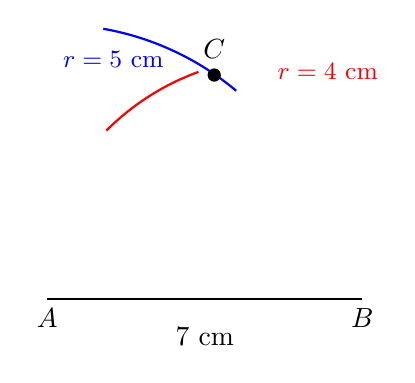
\begin{tikzpicture}[scale=0.8]
  % Base
  \draw[thick] (0,0) -- (5,0);
  \node[below] at (0,0) {$A$};
  \node[below] at (5,0) {$B$};
  \node[below] at (2.5,-0.3) {$7$ cm};
  % Arc from A
  \draw[blue,thick] (3,3.3) arc[start angle=50,end angle=80,radius=4.5];
  \node[blue,left] at (2,3.8) {\small $r = 5$ cm};
  % Arc from B
  \draw[red,thick] (2.4,3.6) arc[start angle=110,end angle=135,radius=4];
  \node[red,right] at (3.5,3.6) {\small $r = 4$ cm};
  % Intersection
  \fill (2.65,3.55) circle (3pt);
  \node[above] at (2.65,3.65) {$C$};
\end{tikzpicture}
\end{center}
\end{questionText}
\choiceA{An equilateral triangle}
\choiceB{A triangle with sides $5$, $4$, and $7$ (SSS)}
\choiceC{A right triangle}
\choiceD{An isosceles triangle with base $7$}
\correctAnswer{B}
\explanation{The base is $7$ cm. An arc of $5$ cm from $A$ and an arc of $4$ cm from $B$ intersect at $C$. This constructs a triangle with sides $5$, $4$, and $7$.}
\end{practiceQuestion}

\begin{practiceQuestion}{m-6-3-q27}{gmc}
\begin{questionText}
The diagram shows three segments. A student claims a triangle can be formed. Is the student correct?

\begin{center}
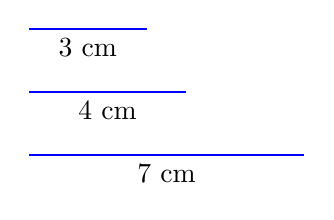
\begin{tikzpicture}
  \draw[thick,blue] (0,0) -- (1.5,0);
  \node[below] at (0.75,0) {$3$ cm};
  \draw[thick,blue] (0,-0.8) -- (2,-0.8);
  \node[below] at (1,-0.8) {$4$ cm};
  \draw[thick,blue] (0,-1.6) -- (3.5,-1.6);
  \node[below] at (1.75,-1.6) {$7$ cm};
\end{tikzpicture}
\end{center}
\end{questionText}
\choiceA{Yes, it is a right triangle}
\choiceB{Yes, all three inequality checks pass}
\choiceC{No, because $3 + 4 = 7$ (not greater than $7$)}
\choiceD{No, because the sides are too different in length}
\correctAnswer{C}
\explanation{$3 + 4 = 7$, which is equal to (not greater than) $7$. The triangle inequality requires the sum to be \textbf{strictly greater}, so no triangle can be formed. The segments would form a straight line instead.}
\end{practiceQuestion}

\begin{practiceQuestion}{m-6-3-q28}{gmc}
\begin{questionText}
The table shows four sets of triangle conditions. Which set does NOT produce a unique triangle?

\begin{center}
\begin{tabular}{|c|l|l|}
\hline
\textbf{Set} & \textbf{Given} & \textbf{Type} \\
\hline
A & Sides: $5$, $7$, $10$ & SSS \\
\hline
B & Sides: $6$, $9$; angle between: $40°$ & SAS \\
\hline
C & Angles: $30°$, $60°$, $90°$ & AAA \\
\hline
D & Angles: $50°$, $80°$; side between: $12$ cm & ASA \\
\hline
\end{tabular}
\end{center}
\end{questionText}
\choiceA{Set A}
\choiceB{Set B}
\choiceC{Set C}
\choiceD{Set D}
\correctAnswer{C}
\explanation{AAA (Set C) fixes the shape but not the size. Many $30$-$60$-$90$ triangles of different sizes exist. Sets A (SSS), B (SAS), and D (ASA) each produce a unique triangle.}
\end{practiceQuestion}

\begin{practiceQuestion}{m-6-3-q29}{gsa}
\begin{questionText}
The diagram shows a failed triangle construction: arcs from each endpoint of an $11$ cm base do not intersect. What does this tell us?

\begin{center}
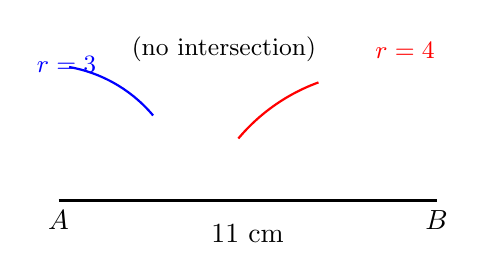
\begin{tikzpicture}[scale=0.6]
  \draw[thick] (0,0) -- (8,0);
  \node[below] at (0,0) {$A$};
  \node[below] at (8,0) {$B$};
  \node[below] at (4,-0.3) {$11$ cm};
  % Arc from A (radius 3 — too short)
  \draw[blue,thick] (2,1.8) arc[start angle=40,end angle=80,radius=3];
  \node[blue,above left] at (1,2.5) {\small $r = 3$};
  % Arc from B (radius 4 — too short)
  \draw[red,thick] (5.5,2.5) arc[start angle=110,end angle=140,radius=4];
  \node[red,above right] at (6.5,2.8) {\small $r = 4$};
  % Gap label
  \node at (3.5,3.2) {\small (no intersection)};
\end{tikzpicture}
\end{center}
\end{questionText}
\correctAnswer{The side lengths $3$, $4$, $11$ do not satisfy the triangle inequality ($3 + 4 = 7 < 11$), so no triangle is possible.}
\explanation{The arcs don't intersect because the two shorter sides ($3$ and $4$) combined are less than the base ($11$). The triangle inequality fails.}
\end{practiceQuestion}

\begin{practiceQuestion}{m-6-3-q30}{gsa}
\begin{questionText}
The diagram shows a valid triangle construction. Identify the construction condition (SSS, SAS, ASA, or AAS) and explain why the triangle is unique.

\begin{center}
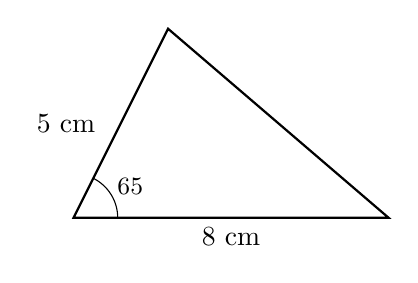
\begin{tikzpicture}[scale=0.8]
  \draw[thick] (0,0) -- (5,0) -- (1.5,3) -- cycle;
  \node[below] at (2.5,0) {$8$ cm};
  \node[left] at (0.5,1.5) {$5$ cm};
  % Angle mark at bottom left
  \draw (0.7,0) arc[start angle=0,end angle=63,radius=0.7];
  \node at (0.9,0.5) {\small $65°$};
\end{tikzpicture}
\end{center}
\end{questionText}
\correctAnswer{SAS — two sides ($8$ cm and $5$ cm) and the included angle ($65°$) determine a unique triangle.}
\explanation{The base is $8$ cm, the left side is $5$ cm, and the angle between them is $65°$. SAS always produces exactly one triangle. The angle and two side lengths fix the position of the third vertex.}
\end{practiceQuestion}
